\documentclass[11pt]{article}
\usepackage[margin=1in]{geometry}
\usepackage{amsmath,amssymb}
\usepackage{graphicx}
\usepackage{float}
\usepackage{xcolor}
\usepackage[hidelinks]{hyperref}
\graphicspath{{figures/}}

% Replace these fields before submitting.
\newcommand{\studentname}{Lukas Hann}
\newcommand{\andrewid}{lukash}
\newcommand{\todo}[1]{\par\noindent\textcolor{blue}{\textbf{TODO:} #1}\par}
\newcommand{\planfigure}[3]{%
  \begin{figure}[H]
    \centering
    \includegraphics[width=0.55\linewidth]{#1}
    \caption{#2}
    \label{#3}
  \end{figure}
}

\title{16-662 Robot Autonomy\\Homework 3}
\author{\studentname\quad (\texttt{\andrewid})}
\date{}

\begin{document}
\maketitle

\section{Symbolic Planning}
% Preserve the assignment numbering after omitting implementation-only sections.
\setcounter{subsection}{2}

\subsection{Planning in Block World}
The generated plan contains three actions.
\planfigure{block-problem-1-plan.png}
  {Generated plan for the first Block World problem (Problem 1.3).}
  {fig:block-world-plan}

\subsection{Another Block World Problem}
The generated plan contains eight actions.
\planfigure{block-problem-2-plan.png}
  {Generated plan for the second Block World problem (Problem 1.4).}
  {fig:block-world-2-plan}

% Problem 1.5 also requires submission of SymPlanner.py and SymScript.py.
% It does not require a separate written answer.

\clearpage
\section{Grasping}

\subsection{Removing Contacts}
\subsubsection*{Grasp matrix}
The origin is at the center of the box, with $+x$ pointing right and $+y$
pointing upward. Positive torque is counterclockwise, and distances are in meters.
For a planar contact at $p_i=(x_i,y_i)$ with force direction
$n_i=(n_{ix},n_{iy})$, use the wrench ordering $(F_x,F_y,\tau_\theta)$:
\[
  g_i=\begin{bmatrix}
    n_{ix}\\ n_{iy}\\ x_i n_{iy}-y_i n_{ix}
  \end{bmatrix},
  \qquad
  G=\begin{bmatrix}g_A & g_B & g_C & g_D & g_E & g_F\end{bmatrix}.
\]
\[
G = \begin{bmatrix}
  0 & 0 & 1 & -1 & 0 & 0 \\
  -1 & -1 & 0 & 0 & 1 & 1 \\
  0.05 & -0.05 & 0 & 0 & -0.05 & 0.05
\end{bmatrix}.
\]

\subsubsection*{Grasp-vector plots}
\begin{figure}[H]
  \centering
  \begin{minipage}{0.49\linewidth}
    \centering
    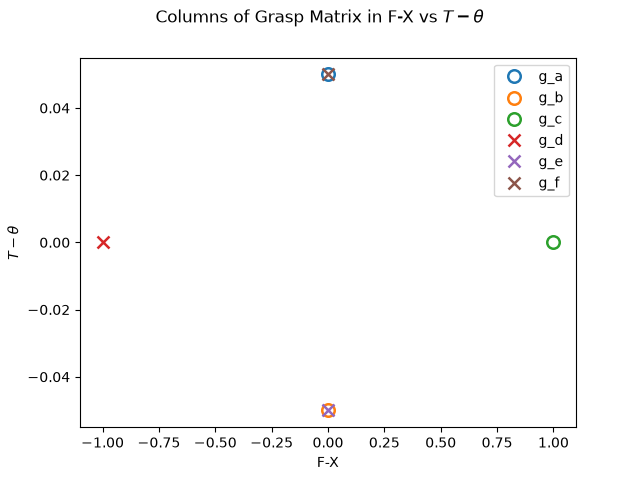
\includegraphics[width=\linewidth]{fx.png}
  \end{minipage}\hfill
  \begin{minipage}{0.49\linewidth}
    \centering
    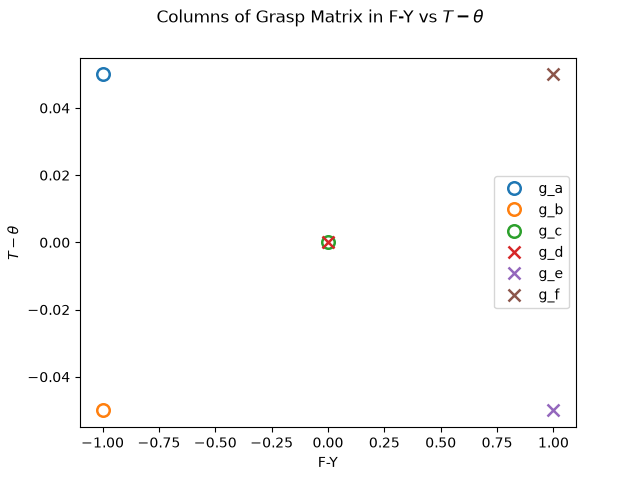
\includegraphics[width=\linewidth]{fy.png}
  \end{minipage}
  \caption{Grasp-vector projections: $F_x$ versus
  $\tau_\theta$ (left) and $F_y$ versus $\tau_\theta$ (right).
  Coincident projections may overlap.}
  \label{fig:grasp-projections}
\end{figure}

\subsubsection*{Removing contacts while preserving form closure}
We cannot remove any contacts and maintain form closure, because form closure requires the columns of G to positively span the wrench space, and figure \ref{fig:grasp-projections} shows that all contacts are required to construct a convex hull that includes the area around the origin.
While the contact pairs A/F and B/E appear redundant in the F-X vs T-$\theta$ diagram, they are not redundant in the F-Y vs T-$\theta$ diagram.

\clearpage
\subsection{Grasp Metrics}
The slanted-edge contacts have Coulomb friction coefficient $\mu=1$;
the shared contact $S$ is frictionless. The requested quality metric is
\[
  Q(G)=\sqrt{\det\!\left(GG^{\mathsf T}\right)}.
\]

\subsubsection*{Coordinate and contact-force conventions}
The origin lies on the triangle's symmetry axis, $0.1\,\mathrm{m}$ above
$S$, with $+x$ pointing right, $+y$ pointing upward, and positive torque
counterclockwise. Each frictional contact is represented by two unit-length
friction-cone edge directions: $(1,0)$ and $(0,-1)$ on the left, and
$(-1,0)$ and $(0,-1)$ on the right. The frictionless contact at $S$ has
direction $(0,1)$. For each grasp $K\in\{A,B,C\}$, the column order is
\[
G_K = \begin{bmatrix}g_S & g_{K1,0} & g_{K1,1} & g_{K2,0} & g_{K2,1}\end{bmatrix}.
\]

\subsubsection*{Grasp A: top-corner contacts}
\[
G_A = \begin{bmatrix}
  0 & 1 & 0 & -1 & 0 \\
  1 & 0 & -1 & 0 & -1 \\
  0 & -0.1 & 0 & 0.1 & 0
\end{bmatrix}.
\]
\[
G_AG_A^{\mathsf T} = \begin{bmatrix}
  2 & 0 & -0.2 \\ 0 & 3 & 0 \\ -0.2 & 0 & 0.02
\end{bmatrix},
\qquad Q_A = \sqrt{0}=0.
\]

\subsubsection*{Grasp B: midpoint contacts}
\[
G_B = \begin{bmatrix}
  0 & 1 & 0 & -1 & 0 \\
  1 & 0 & -1 & 0 & -1 \\
  0 & 0 & 0.1 & 0 & -0.1
\end{bmatrix}.
\]
\[
G_BG_B^{\mathsf T} = \begin{bmatrix}
  2 & 0 & 0 \\ 0 & 3 & 0 \\ 0 & 0 & 0.02
\end{bmatrix},
\qquad Q_B = \sqrt{0.12}\approx 0.346410.
\]

\subsubsection*{Grasp C: bottom-corner contacts}
\[
G_C = \begin{bmatrix}
  0 & 1 & 0 & -1 & 0 \\
  1 & 0 & -1 & 0 & -1 \\
  0 & 0.1 & 0.2 & -0.1 & -0.2
\end{bmatrix}.
\]
\[
G_CG_C^{\mathsf T} = \begin{bmatrix}
  2 & 0 & 0.2 \\ 0 & 3 & 0 \\ 0.2 & 0 & 0.1
\end{bmatrix},
\qquad Q_C = \sqrt{0.48}\approx 0.692820.
\]

\subsubsection*{Best grasp}
According to the grasp metric $Q(G)$ Grasp C is the best grasp because it produces the largest score. Using this score, grasp C wins because $G_A$ has rank two, and therefore a score of zero, and grasp C beats grasp B because grasp C has a larger moment arm.

% Submission checklist (not printed):
% 1. Replace name/Andrew ID and complete/remove all TODOs.
% 2. Verify both included Block World plan screenshots.
% 3. Compile and name the final PDF andrewid_hw3_16662.pdf.
% 4. Package the code as andrewid_hw3_code_16662.zip, including the required
%    SymPlanner.py and SymScript.py files. Exclude venv/conda environments.
% 5. Put the code zip and PDF inside andrewid_hw3_16662.zip.
\end{document}
